\documentclass[a4paper]{article}

\usepackage[utf8]{inputenc}
\usepackage{polski}
\usepackage[polish]{babel}
\usepackage[margin=1in]{geometry}
\usepackage{lmodern}
\usepackage{tabularx}
\usepackage{graphicx}
\usepackage{hyperref}
\usepackage{float}
\newcounter{counter}
\newcommand\rownumber{\stepcounter{counter}\arabic{counter}}

\hypersetup{
    colorlinks,
    citecolor=black,
    filecolor=black,
    linkcolor=black,
    urlcolor=black
}

\title{\textbf{Podsumowanie prac z projektu WDS - kwiecień 2015}}
\author{Marcin Ochman - 200546}
\date{}
\begin{document}


\begin{titlepage}
\begin{center}

 \newcommand{\HRule}{\rule{\linewidth}{0.5mm}}
%\includegraphics[width=0.15\textwidth]{./logo}~\\[1cm]

\textsc{\Large Projekt z Wizualizacji danych sensorycznych}\\[1cm]

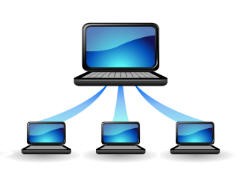
\includegraphics{network_icon}


\HRule \\[0.4cm]
{ \huge \bfseries \textit{Computer Monitor} - monitorowanie komputerów poprzez sieć.\\[0.4cm] }

{\huge \underline{\textit{Raport postępu prac }}}\\[0.5cm]


\LARGE 23.04.2015
\HRule \\[1.5cm]


\noindent
\begin{minipage}[t]{0.4\textwidth}
\begin{flushleft} \large
\emph{Autor:}\\
Marcin \textsc{Ochman}
\end{flushleft}
\end{minipage}%
\begin{minipage}[t]{0.4\textwidth}
\begin{flushright} \large
\emph{Prowadzący} \\
Dr inż. Bogdan \textsc{Kreczmer}
\end{flushright}
\end{minipage}


\end{center}
\end{titlepage}

\newpage

\tableofcontents
\listoffigures
\listoftables

\newpage

	\section{Założenia projektowe}
		Celem projektu było napisanie aplikacji \textit{,,Computer Monitor''} przeznaczoną na komputery osobiste, która:
	\begin{itemize}
		\item pozwala na monitorowanie pracy komputera(ów), z którym(i) komputer jest połączony poprzez sieć
		\item pracuje w różnych trybach:
		\begin{itemize}
			\item tryb wizualizacji
			\item tryb raportowania
			\item połączenie dwóch poprzednich trybów
		\end{itemize}
		\item potrafi zapamiętać ustawienia użytkownika, w tym m.in. tryb działania aplikacji, układy okien, ustawienia wykresów itp.
		\item posiada przejrzysty, intuicyjny, atrakcyjny oraz konfigurowalny interfejs użytkownika rozumiany w następujący sposób:
		\begin{itemize}
			\item będą wyraźnie zaznaczone różne kategorie monitorowanych wielkości np. procesor, karta graficzna, pamięć \uppercase{ram}
			\item zaimplementowanie animacji
			\item dostosowywanie wykresów np. jego wielkość
			 
		\end{itemize}
		\item pomimo realizowanej komunikacji poprzez sieć oraz innych zadań, jest wysoce 
		interaktywna
		\item docelową platformą jest system Linux, jednak zostaną poczynione wszelkie starania, aby aplikacja działała również na systemach Windows
	\end{itemize}
	
	\section{Opis poszczególnych trybów pracy}
	Poniżej zostały opisane poszczególne tryby pracy aplikacji.
	
	\subsection{Tryb wizualizacji}
		W tym trybie program prezentuje dane, które są pobierane poprzez sieć. Pozwala na śledzenie wartości poszczególnych wielkości opisujących stan komputera oraz prezentowanie danych na wykresach (zależności czasowe, zużycie zasobów komputera np. w formie wykresu kołowego) oraz diagramach/ilustracjach (monitorowanie i alarmowanie poprawności funkcjonowania systemu). Progi alarmowe można również zdefiniować samodzielnie. Dodatkowo będzie możliwość zapisywania raportów zawierających dane zdobyte w trakcie monitorowania.
	
	\subsection{Tryb raportowania}
		Program działający w trybie raportowania ma za zadanie śledzenie pracy komputera oraz wysyłanie zebranych informacji poprzez sieć. Użytkownik ma możliwość wyboru danych, które zostaną wysłane. Aplikacja będzie działać w systemowym zasobniku.
	
	\subsection{Tryb łączony}
		Jest to połączenie dwóch poprzednich trybów. Pozwala na jednoczesne wizualizowanie aktualnego stanu komputera, na którym została uruchomiona aplikacja oraz wysyłanie zebranych informacji poprzez sieć. Dwa ostatnie tryby zostały wyodrębnione ze względu na umożliwienie optymalizacji zasobów zajmowanych przez aplikację.
	


\section{Wstęp raportu}

W ciągu miesiąca, tj. 23.04.2015-14.05.2015, zostało wykonanych wiele prac nad aplikacją. W tym dokumencie opisano wykonane i przewidywane na następny miesiąc zadania oraz komentarz autora na temat postępów prac nad aplikacją.

\section{Lista wykonanych zadań w projekcie}

\subsection{Pierwszy termin kontrolny prac nad aplikacją - wstępne rezultaty}
W poniższej tabeli zostały zebrane zadania, które udało się zrealizować do dnia 23.04.2015r.

\begin{table}[h]
\centering
\begin{tabularx}{0.7\linewidth}{ |c|X| }
			\hline 
			\rownumber & Opracowano architekturę aplikacji - użyte biblioteki oraz 
						 klasy do napisania\\ \hline
			\rownumber & Utworzono strukturę katalogów aplikacji \\ \hline
			\rownumber & Aplikacja buduje się przy pomocy wieloplatformowego narzędzia 
						 \textit{CMake} - napisanie plików potrzebnych do poprawnej kompilacji \\ \hline
			\rownumber & Rozpoczęto pracę nad biblioteką \textit{SystemMonitoringLib} \\ \hline
			\rownumber & Rozpoczęto pracę nad interfejsem użytkownika \\ \hline
			\rownumber & Rozpoczęta pracę nad komunikacją pomiędzy biblioteką \textit{SystemMonitoringLib} oraz interfejsem użytkownika \\ \hline
	\end{tabularx}
	\caption{Tabela prac nad aplikacją}
\end{table}

\subsection{Drugi termin kontrolny prac nad aplikacją - rezultaty prawie końcowe}

\section{Szczegółowy opis wykonanych zadań}

\subsection{Pierwszy termin kontrolny prac nad aplikacją - wstępne rezultaty}

\subsubsection{Opracowanie architektury aplikacji}
Program będzie opierać się na bibliotekach \textit{Qt5} i \textit{QCustomPlot}, które posłużą do prezentacji danych oraz autorskiej biblioteki, która została opisane w następnych punktach - \textit{SystemMonitoringLib}. Biblioteki monitorujące będą komunikować się z warstwą prezentacji za pomocą odpowiedniej klasy pośredniczącej. Diagram budowy aplikacji został przedstawiony na rysunku \ref{diagram_budowy_aplikacji},  diagram klas został przedstawiony na rysunku \ref{diagram_klas}, a diagram przypadków użycia na rysunku \ref{diagram_przypadkow_uzycia}.

\begin{figure}[H]
	\centering
	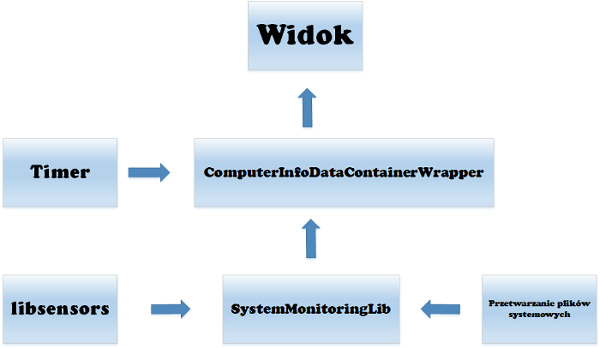
\includegraphics[width=\linewidth]{img/diagramBudowyAplikacji.png}
	\caption{Diagram budowy aplikacji}
	\label{diagram_budowy_aplikacji}
\end{figure}


\begin{figure}[H]
	\centering
	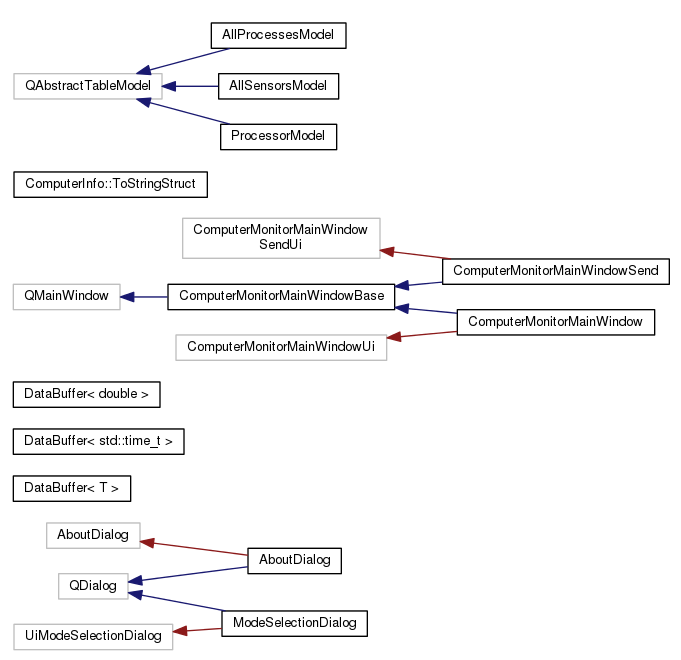
\includegraphics[width=\linewidth]{img/diagramKlas.png}
	\caption{Diagram UML stworzonych klas (1)}
	\label{diagram_klas}
\end{figure}

\begin{figure}[H]
	\centering
	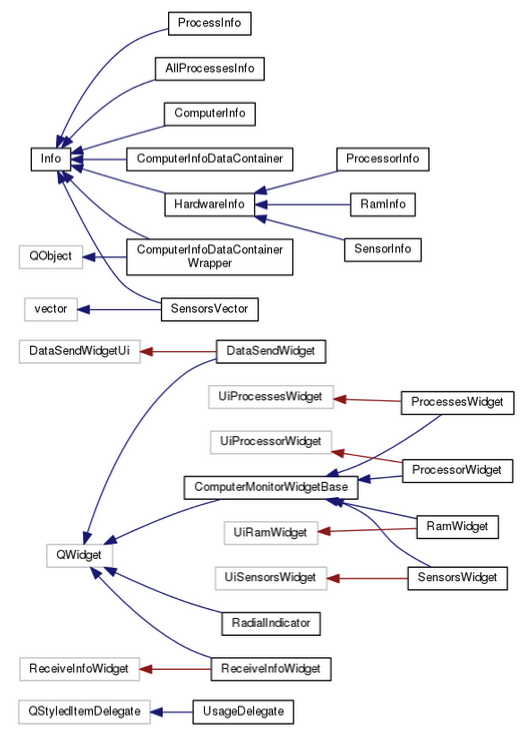
\includegraphics[width=\linewidth]{img/diagramKlas2.png}
	\caption{Diagram UML stworzonych klas (2)}
	\label{diagram_klas_2}
\end{figure}

\begin{figure}[H]
	\centering
	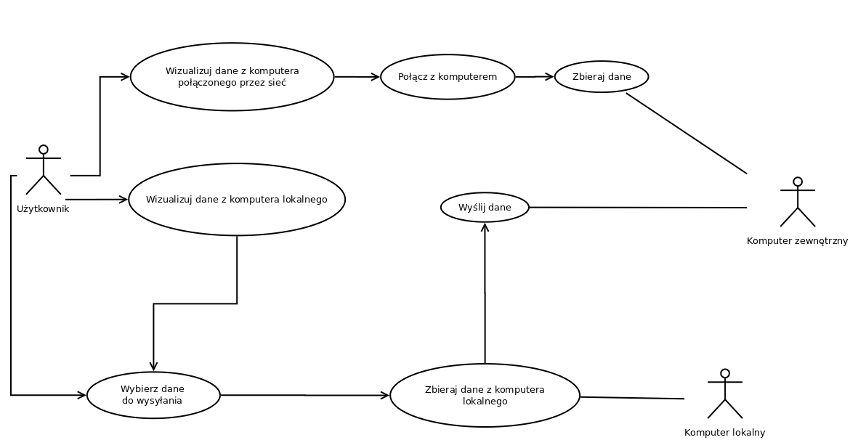
\includegraphics[width=0.75\paperheight, angle=90]{img/diagramPrzypadkowUzycia.png}
	\caption{Diagram przypadków użycia}
	\label{diagram_przypadkow_uzycia}
\end{figure}

\subsubsection{Stworzenie zalążka aplikacji}

Zalążek aplikacji wymagał kilku pomniejszych kroków do wykonania:
\begin{itemize}
	\item utworzenie struktury folderów projektu
	\item napisanie skryptów kompilujących i konsolidujących
\end{itemize}
Opis poszczególnych zadań znajduje się poniżej.

\subsubsection{Struktura folderów projektu}
W głównym folderze aplikacji znajdują się dwa foldery: \textit{doc} oraz \textit{prj}. Pierwszy zawiera wszelkie pliki przechowujące informacje o dokumentacji, a drugi zawiera kody źródłowe aplikacji. W folderze \textit{prj} można wyróżnić kilka folderów. Ich krótki opis zebrano w tabeli \ref{opis_folderow_prj}.

\begin{table}
\centering
\begin{tabularx}{0.7\linewidth}{|c|X|}
	\hline
	inc & przechowuje wszystkie pliki nagłówkowe, które nie należą do bibliotek\_l \\ \hline
	src & zawiera pliki źródłowe, które nie należą do bibliotek \\ \hline
	lib & przechowuje pliki źródłowe oraz nagłówkowe bibliotek, każda biblioteka jest umieszczona 
		  w innym folderze. W każdym z folderów są pliki nagłówkowe oraz źródłowe \\ \hline
	ui & znajdują się w nim wszystkie pliki  programu QtDesigner \\ \hline
	rsrc  & zawiera zasoby aplikacji \\ \hline
\end{tabularx}
\caption{Opis poszczególnych folderów w katalogu \textit{prj/}}
\label{opis_folderow_prj}
\end{table}

\subsubsection{Proces kompilacji oraz opis narzędzia \textit{CMake}}
Program \textit{CMake} to wieloplatformowy system do budowania aplikacji. Dzięki niemu łatwe staje się
znajdowanie odpowiednich plików nagłówkowych oraz bibliotek oraz kompilacja na różnych platformach (m.in. Linux i Windows). Każdy folder zawiera w sobie plik \textit{CMakeLists.txt}, który definiuje w jaki sposób ma zachować się program budujący.Dzięki niemu, oszczędzono wiele czasu na kompilację oraz konsolidację programu używającego bibliotek \textit{Boost} oraz \textit{Qt5}. Najpierw budowane są biblioteki, a następnie cały program. Wszystko zostaje skonsolidowane. Istnieje również możliwość wygenerowania dokumentacji, wystarczy, że zbudujemy cel \textit{doc}.

\subsubsection{Biblioteka \textit{SystemMonitoringLib}}
Jest to biblioteka do monitorowania lokalnego komputera oraz wysyłania informacji przez sieć. Pozwala na pobieranie odczytów z czujników, informacji o procesorze takich jak częstotliwość taktowania poszczególnych rdzeni, zużycie procesora, o pamięci RAM (dostępna pamięć, zużycie) oraz informacje o poszczególnych procesach. Na komputerze z uruchominionym systemem \textit{Linux}, biblioteka do zbierania informacji o komputerze używa innej biblioteki - \textit{sensorslib} oraz przetwarze pliki m.in. \textit{/proc/stat/}, \textit{/proc/cpuinfo}

\subsubsection{Interfejs użytkownika}
Roczpoczęto prace nad wizualizowaniem danych  odczytanych z czujników dostępnych na płycie głównej.
W widoku tabelki mamy możliwość podglądania aktualnych wartości odczytanych wielkości. Zrzut ekranu przedstawiającego aktualny stan interfejsu użytkownika został pokazany na rysunku \ref{wygladAplikacji}.

\subsection{Drugi termin kontrolny prac nad aplikacją - rezultaty prawie końcowe}

\subsubsection{Dokończenie prac nad biblioteką do monitorowania komputera}

Zostały poczynione duże kroki w tym kierunku. Dodano klasy \texttt{ProcessInfo}, \texttt{ProcessorInfo}, \texttt{RamInfo} oraz \texttt{AllProcessesInfo}. Są one odpowiedzialne za śledzenie procesów, informacji o procesorze, informacji o pamięci
RAM oraz informacji o wszystkich procesach. Biblioteka została napisana na system Linux. Nie jest kompatybilna na komputerach z systemem Windows, tak jak zakładano to na samym początku. 

\subsubsection{Kontynuacja implementacji interfejsu użytkownika}

Zaimplementowanie wielu funckjonalności biblioteki \textit{SystemMonitoringLib} umożliwiło dalszą implementację
prezentacji danych zebranych przez tę bibliotekę w przejrzysty i atrakcyjny dla oka sposób. Postanowiono, że aplikacja
będzie mieć spójny interfejs dla każdego monitorowanego komponentu. Dzięki temu możemy zobaczyć, że każda strona ma podobny wygląd - po lewej stronie mamy do wyboru element poszczególnego komponentu (np. dla procesora jest to rdzeń). Po prawej stronie mamy wykres monitorowanej wielkości, którą możemy wybrać (jeśli jest taka możliwość) za pomocą listy rozwijalnej. Wygląd aplikacji został przedstawiony na rysunku \ref{wygladAplikacji}.

\subsection{Termin oddania}

% % % % % % % % % % % % % % % % % % % % % % % % % % % % % % %5

W ostatnim miesiącu pracy nad projektem aplikacja bardzo się rozwinęła. Poniżej przedstawiono, co zostało wykonane.

\subsubsection{Biblioteka \textit{SystemMonitoringLib}}
W autorskiej bibliotece monitorującej komputer musiałem wprowadzić poprawki, aby przystosować ją
do pracy w sieci. 

\subsubsection{Interfejs użytkownika}
Interfejs użytkownika uległ bardzo wielu zmianom. Został on wzbogacony o:
\begin{itemize}
	\item analogowy zegar pokazujący zużycie procesora
	\item lepsza prezentacja danych tabelarycznych
	\item możliwość wyboru i zapamiętywanie palety kolorów
	\item kontrolki ustawień połączeń sieciowych
	\item w trybie raportowania możliwość minimalizacji okna do systemowego zasobnika
\end{itemize}

\subsubsection{Połączenie sieciowe}
Zaimplementowano dwa rodzaje połączeń. Pierwsze z nich to połączenie do serwera, który wysyła dane. Drugie to postawienie serwera i wysyłanie informacji o komputerze do klienta.


\begin{figure}[H]
	\centering
	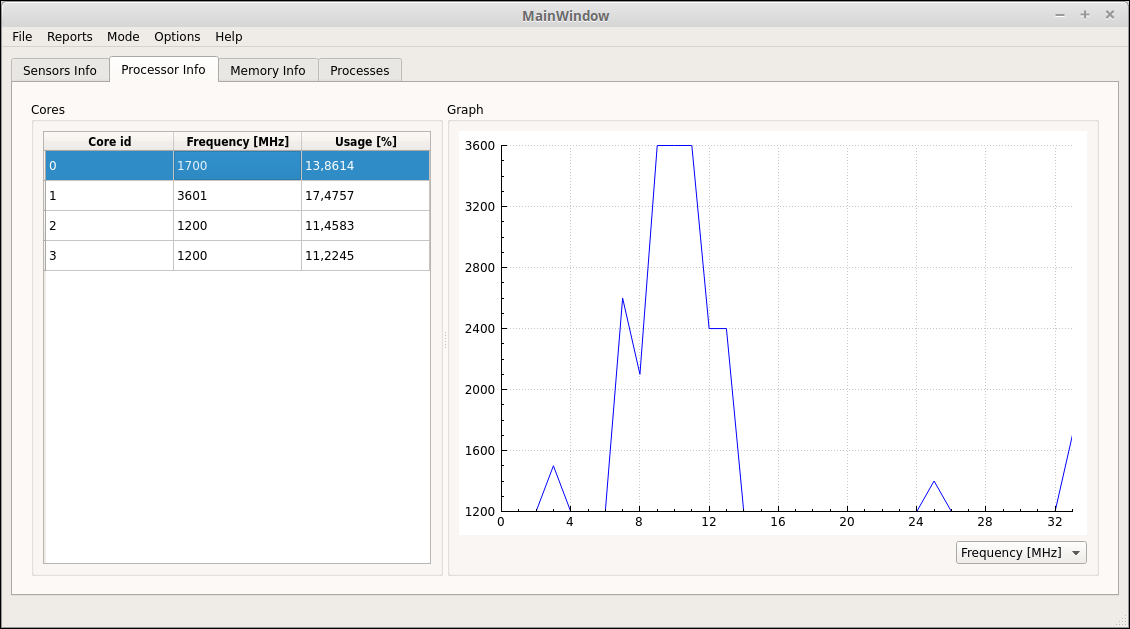
\includegraphics[width=\linewidth]{img/wygladAplikacji.png}
	\caption{Wygląd aplikacji \textit{ComputerMonitor}}
	\label{wygladAplikacji}
\end{figure}



% % % % % % % % % % % % % % % % % % % % % % % % % % % % % % % %

\section{Opis zrealizowanych, planowanych i zaniechanych funkcjonalności}

Poniżej zostały opisane wszystkie funkcjonalności aplikacji, które na początku istnienia projektu
miały zostać zaimplementowane, jednak ze względu na ograniczenia czasowe zostały porzucone.

\subsection{Pierwszy termin kontrolny prac nad aplikacją - wstępne rezultaty}

Na dzień 23.04.2015 została zrealizowana funkcjonalność wizualizacji danych z czujników. Planowane funkcjonalności nie zmieniły się - są zgodne z tym co można znaleźć w założeniach projektu. Niestety ze względu na niedostateczną ilość czasu wersja na system \textit{Windows} została wstrzymana.

\subsection{Drugi termin kontrolny prac nad aplikacją - rezultaty prawie końcowe}
Na dzień 14.05.2015r została zrealizowana funkcjonalność wizualizacji \textsc{wszystkich} komponentów monitorowanych przez bibliotekę \textit{SystemMonitoringLib}:
	\begin{itemize}
		\item Procesor
		\item Pamięć \textsc{RAM}
		\item Uruchomione procesy
		\item Czujniki
	\end{itemize}
Oznacza to, że zostały zakończone prace nad biblioteką \textit{SystemMonitoringLib} oraz wykonano wiele pracy nad interfejsem użytkownika.


\subsection{Termin oddania}
Na dzień 11.06.2015r została zrealizowana ostatnia część implementacyjna programu:
	\begin{itemize}
		\item połączenie sieciowe
		\item interfejs użytkownika
	\end{itemize}
Oznacza to, że prace nad aplikacją zostały ukończone w zadowalającym stopniu. 
Niestety nie udało się w większym stopniu zaimplementować zapisywania ustawień użytkownika. Jest to jedyna
część programu, która nie została zrealizowana w taki sposób, jak zaplanowano.



\section{Opis interfejsu użytkownika}

Aplikacja na samym początku pokazuje okienko wyboru trybu aplikacji, które zostało pokazane na rysunku \ref{okno_wyboru_trybu}. Mamy do wyboru trzy tryby:
\begin{itemize}
			\item tryb wizualizacji
			\item tryb raportowania
			\item tryb łączony
\end{itemize}
W każdym z trybów jest możliwość wyświetlenia informacji o autorze oraz zmiany palety kolorów.

\begin{figure}[H]
	\centering
	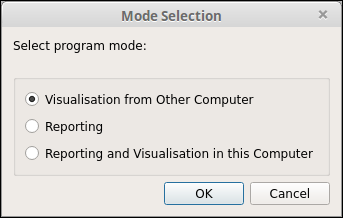
\includegraphics[height=0.15\paperheight]{img/oknoWyboruTrybu.png}
	\caption{Wygląd aplikacji \textit{ComputerMonitor}}
	\label{okno_wyboru_trybu}
\end{figure}


\subsection{Tryb wizualizacji}
W tym trybie są prezentowane dane pobierane z innego komputera. Mamy do wyboru pięć zakładek:

\begin{itemize}
	\item \textit{Sensor Info} - widok odpowiedzialny za czujniki
	\item \textit{Processor Info} - widok odpowiedzialny za procesor
	\item \textit{Ram Info} - widok odpowiedzialny za pamięć operacyjną
	\item \textit{Processes Info} - widok odpowiedzialny za wszystkie procesy
	\item \textit{Server Config} - widok odpowiedzialny za połączenie z serwerem
\end{itemize}
Istnieje możliwość wyeksportowania aktualnie widocznego wykresu przy pomocy \textit{File}$\rightarrow$\textit{Export Plot}. Widok tego trybu został przedstawiony na rysunku \ref{okno_trybu_wizualizacji}.

\begin{figure}[H]
	\centering
	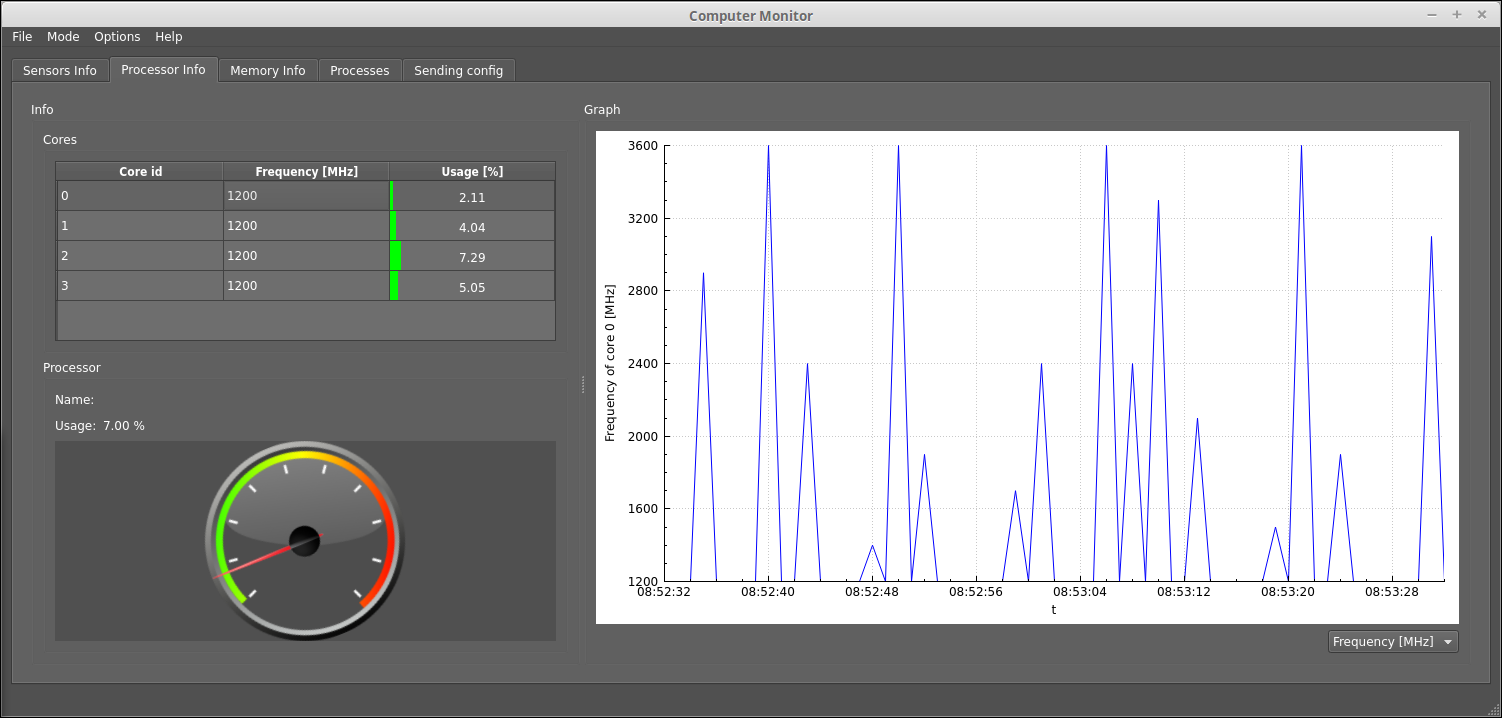
\includegraphics[height=0.25\paperheight]{img/oknoTrybuWizualizacji.png}
	\caption{Okno trybu wizualizacji}
	\label{okno_trybu_wizualizacji}
\end{figure}

\subsection{Tryb raportowania}
W tym trybie mamy jedynie możliwość uruchomienia serwera o określonych parametrach. W polach Ip address oraz Port możemy wpisać namiary klienta, do którego będziemy wysyłać dane. Ciekawostką jest zaimplementowanie ikony zasobnika systemy. Jeśli zminimalizujemy program w tym trybie, to program ukryje się i będzie działać w zasobniku.

\begin{figure}[H]
	\centering
	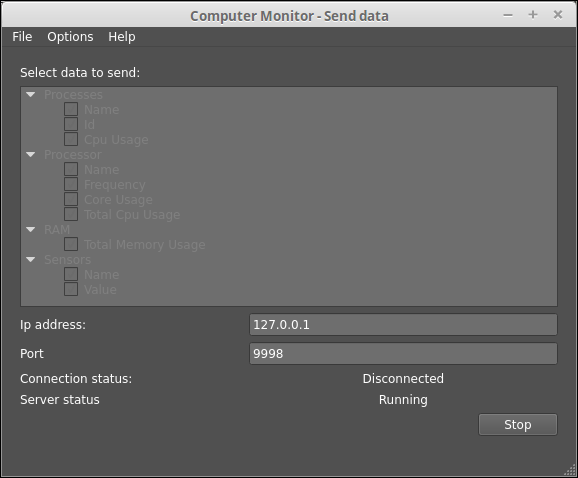
\includegraphics[height=0.25\paperheight]{img/oknoTrybuRaportowania.png}
	\caption{Okno trybu raportowania w trakcie uruchomienia serwera}
	\label{okno_trybu_raportowania}
\end{figure}

\subsection{Tryb łączony}

Jak sama nazwa wskazuje, tryb łączony, jest połączeniem dwóch poprzednich trybów. Został on przedstawiony na rysunku. Została dodana zakładka ,,Sending config'' do konfiguracji parametrów wysyłania.

\begin{figure}[H]
	\centering
	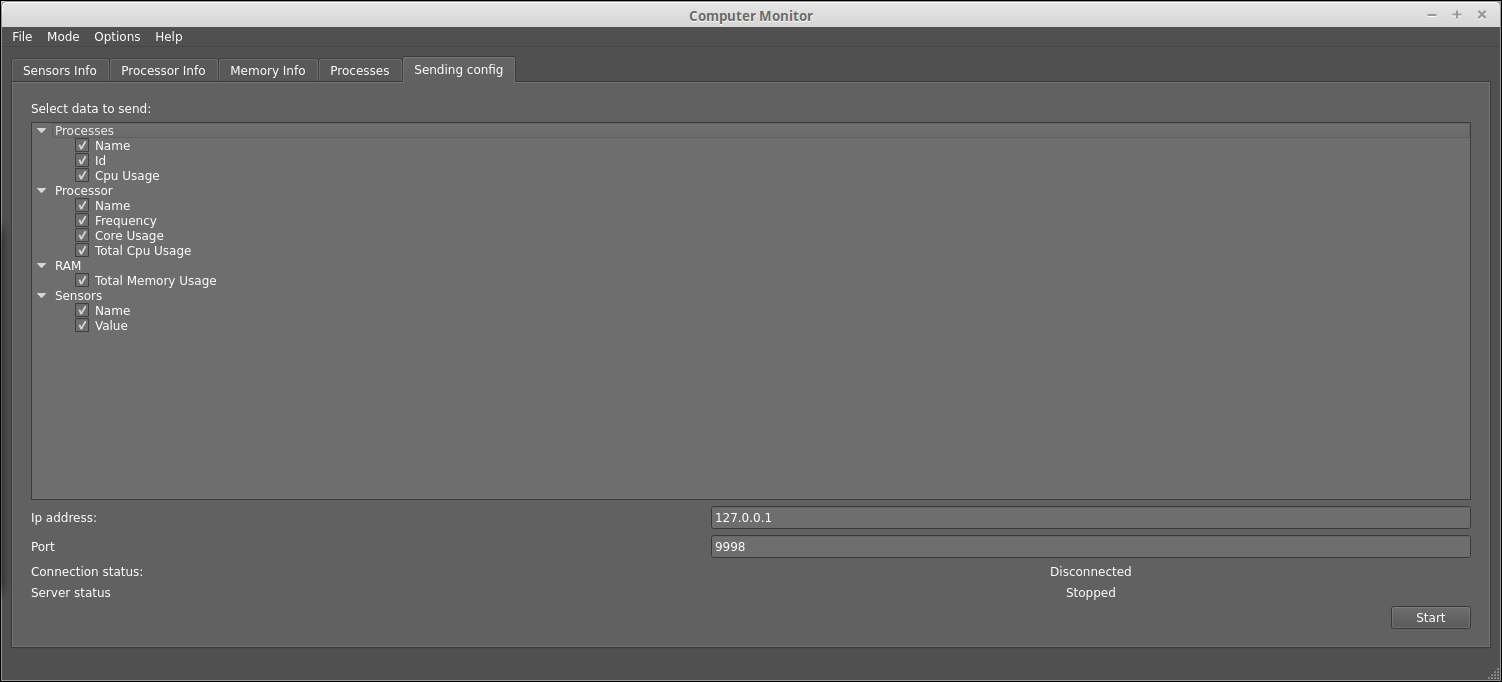
\includegraphics[height=0.25\paperheight]{img/oknoTrybuLaczonego.png}
	\caption{Okno trybu łączonego}
	\label{okno_trybu_laczonego}
\end{figure}


\section{Przykład pracy aplikacji}

Po uruchomieniu dwóch instancji programu w różnych trybach tj. w trybie raportowania oraz w trybie wizualizacji, wygenerowałem wykres, który został przedstawiony na rysunku \ref{wykres_aplikacja}. Prezentuje on taktowanie procesora podczas uruchomienia programu \texttt{stress}. Widać na wykresie, że częstotliwość rdzenia zmienia się razem z obciążeniem systemu. Okres, kiedy częstotliwość taktowania procesora wynosi 3600 \textit{MHz} to okres, w którym działał program \texttt{stress}.

\begin{figure}[H]
	\centering
	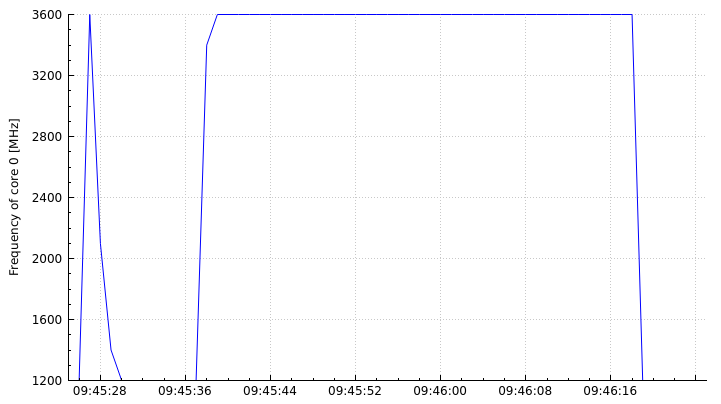
\includegraphics[height=0.25\paperheight]{img/wykres.png}
	\caption{Wyeksportowany wykres do pliku \textit{.png}}
	\label{wykres_aplikacja}
\end{figure}

\section{Podsumowanie}

Praca nad aplikacją \textit{ComputerMonitor} dała mi duże doświadczenie z biblioteką \textit{Qt5}. Poznałem również podstawy programowania sieciowego. Po semestrze starań, mogę stwierdzić, że jestem zadowolony z uzyskanych efektów. Największy problem stanowił połączenie wszystkich danych z widokiem aplikacji, ale ostatecznie udało się to wykonać. Aplikacja spełnia swoje zadanie. Myślę, że w wolnej chwili będę ją dalej rozwijał.
\end{document}